%!TEX root = ../../architekturdokumentation.tex
\chapter{Systemübersicht}
	\begin{wrapfigure}[8]{R}{0.5\textwidth}
  		\vspace{-25pt}
	  	\begin{center}
    		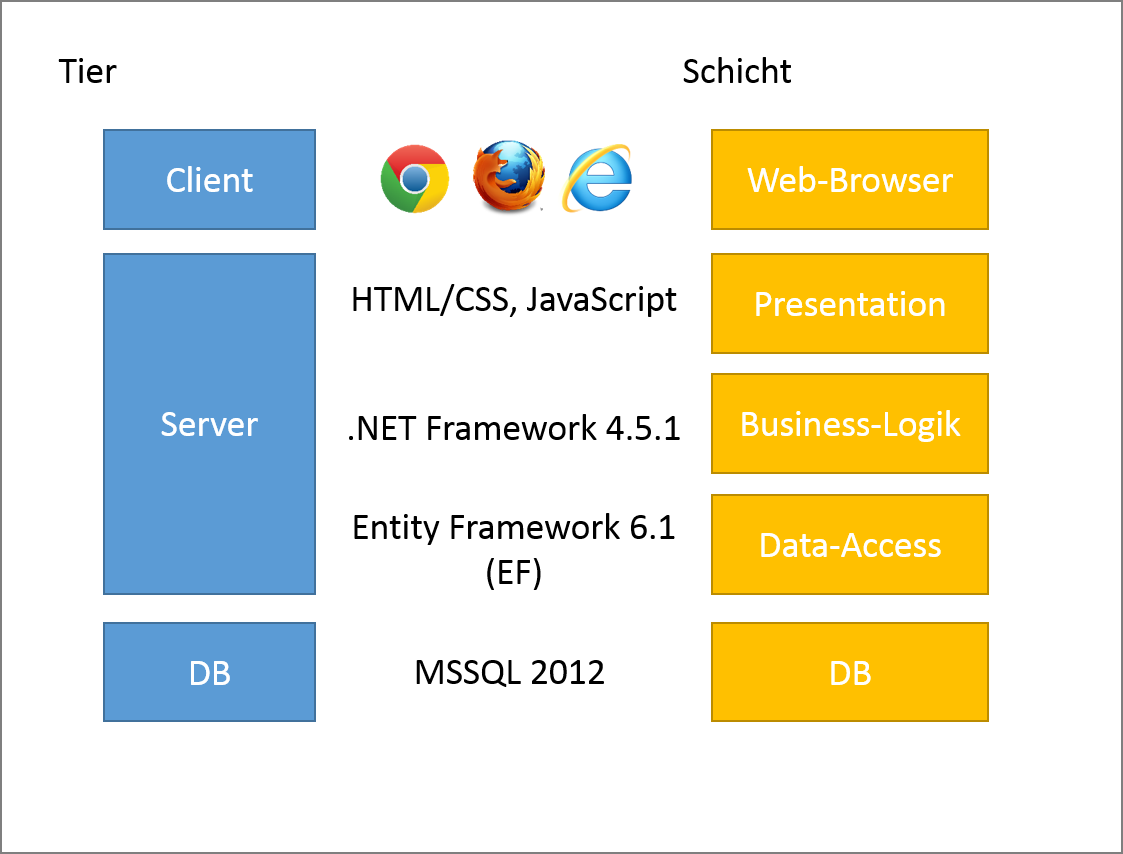
\includegraphics[height=7cm]{content/architekturdokumentation/images/systemarchitektur.png}
	  	\end{center}
  		\vspace{-20pt}
	 	\caption{Systemübersicht von VoluntaryO}
	\end{wrapfigure}
    Diese Darstellung soll als Big-Picture üder die verwendeten Technologien nach Tier dienen.
	Die Systemarchitektur von VoluntaryO gliedert sich in drei Teilbereiche: 
	\\\begin{itemize}
		\item die Datenbank
		\item die Serviceschnittstelle
		\item die Presentationschicht
	\end{itemize}
  	\vspace{3cm}

	\section{Komponenten}
		\subsection{Datenbank}
		Als Datenbanksystem wird der Microsoft SQL Server 2012 eingesetzt. Auf den Entwicklungsmaschinen setzen wir die in Visual Studio eingebaut LocalDb ein. Die Datenbank wird über SQL Management Studio administriert. Der Grund für die Evaluation des SQL Servers ist die gute Integration in die Microsoft Umgebungen. Das Entity Framework (EF) sollte aber einen einfachen Austausch des Datenbank Systems ermöglichen.
		\subsection{Webserver}
		Als Webserver setzen wir den Internet Information Server (IIS) von Microsoft ein, der uns bestmögliche Integration in unsere Entwicklungsumgebung bieten soll. Auf den Entwicklungsmaschinen ist IIS Express installiert, dass standardmässig mit Visual Studio ausgeliefert wird.
		\subsection{Client}
		Die späteren Benutzer werden über einen Webbrowser auf die Applikation zugreifen. Unsere Applikation soll heute gängige Browser unterstützen. Konkret werden wir hier die von Bootstrap 3.0 unterstützten Browser supporten. Mobile Browser werden nicht direkt getestet aber unterstützt. Einzig die Anmeldung für einen Event sollte auch per Mobile Browser möglich sein.

	\section{Schnittstellen}
	    \begin{figure}[h]
	  		\vspace{-5pt}
	    	\centering
	    	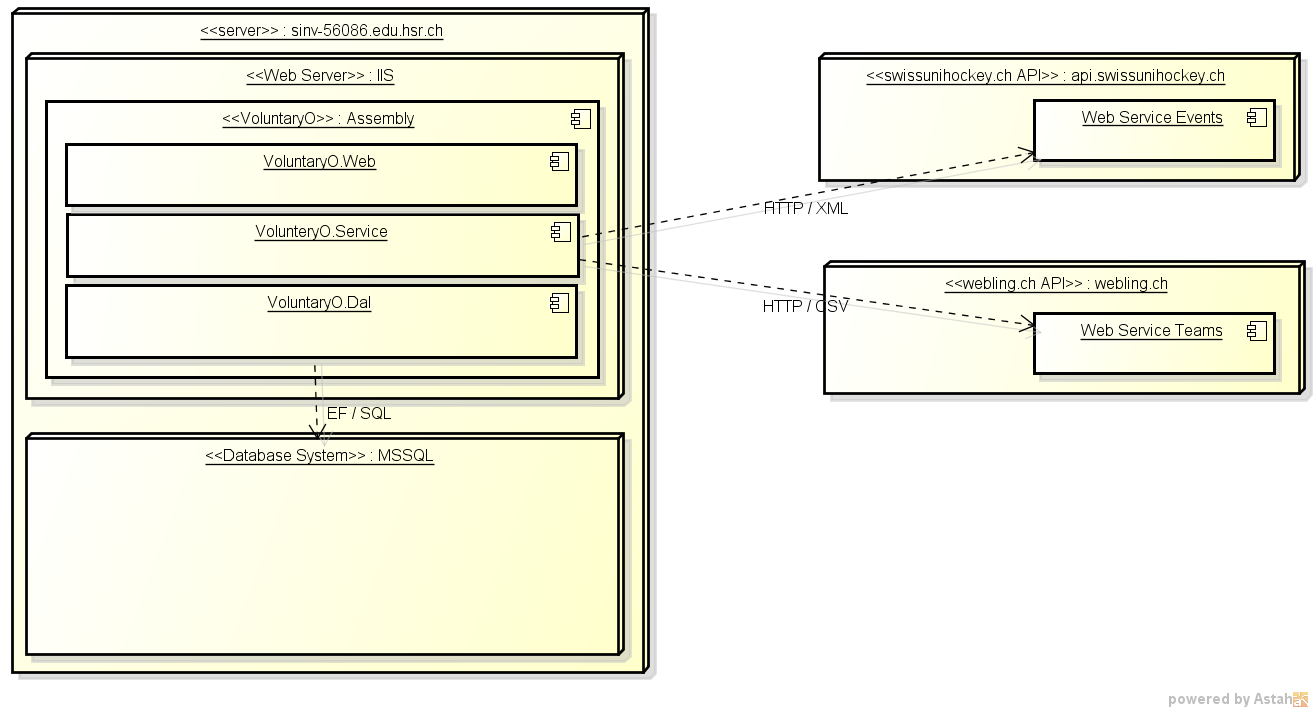
\includegraphics[width=0.9\textwidth]{content/architekturdokumentation/images/uebersicht_der_komponenten.png}
	  		\vspace{-25pt}
	    	\caption{Übersicht der Komponenten und Schnittstellen}
		\end{figure}

		\subsection{Datenbankzugriff}
		Der Datenbankzugriff erfolgt direkt über das Entity Framework (EF). Hier werden die Abfragen über LINQ erstellt.

		\subsection{Webling CSV}
		Die Schnittstelle auf die Vereinsverwaltung Webling soll die Möglichkeit bieten auf Benutzer und Team Informationen zuzugreifen. Die Daten werden in einem CSV-File angeboten, welches mittels eines HTTP-GET in unsere Applikation geladen wird.
		\\Die Webling Schnittstelle ist hier dokumentiert: 
		\\\url{http://doku.webling.ch/about/mitgliederverwaltung/#mit_schnittstelle}

		\subsection{Swissunihockey REST}
		Swissunihockey ist ebenfalls eine externe Schnittstelle, welche die aktuellen Events anbietet. Hier kann auf die Daten über eine REST-API zugegriffen werden.
		\\Die Swissunihockey REST Schnittstelle ist hier dokumentiert: 
		\\\url{http://api.swissunihockey.ch/restendpoints}